\documentclass{article}
\usepackage[utf8]{inputenc}
\usepackage[a4paper, total={15cm, 24cm}]{geometry}
\usepackage{caption}
\usepackage{subcaption}
\usepackage{graphicx}
\usepackage{indentfirst}
\usepackage{sectsty}
\usepackage{longtable}
\usepackage{booktabs}% http://ctan.org/pkg/booktabs
\newcommand{\tabitem}{~~\llap{\textbullet}~~}
\usepackage[table]{xcolor}% http://ctan.org/pkg/xcolor
% \usepackage[table,xcdraw]{xcolor}

\sectionfont{\fontsize{13}{15}\selectfont}
\subsectionfont{\fontsize{10}{12}\selectfont}

\title{Analysis of experiments with modifications on the datasets}

\author{Group on Interactive Coding of Images\\ \\
Department of Information and Communications Engineering\\ \\
Universitat Autònoma de Barcelona}
\date{}


\begin{document}

\maketitle


\section*{Introduction}
\begin{enumerate}
    \item This document shows the obtained results when applying different modifications on the original dataset in order to take advantadge on the correlation of the data. The realized experiments are described as: 
        \subitem- \textbf{Original:} original corpus of images.
        \subitem- \textbf{Bands:} each image is splited in the four bands.
        \begin{figure}[h!]
    \centering
    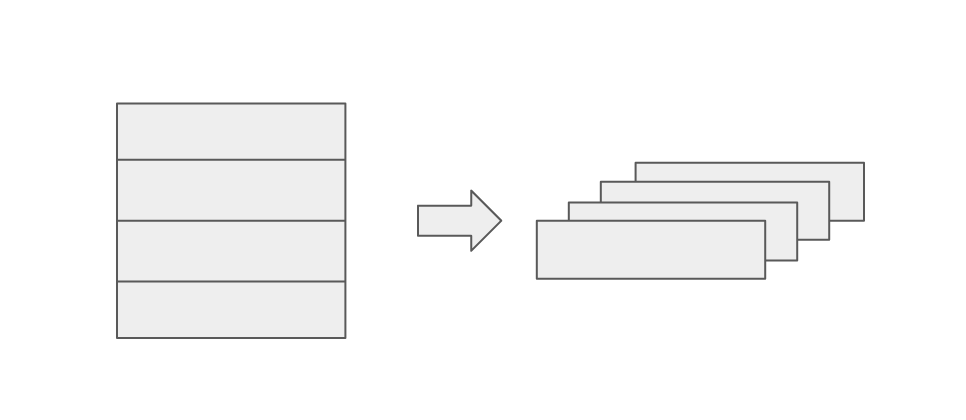
\includegraphics[scale=0.3]{img_1.png}
\end{figure}
        \subitem- \textbf{Moving Bands:} bands of consecutive images are stacked.
        \begin{figure}[h!]
    \centering
    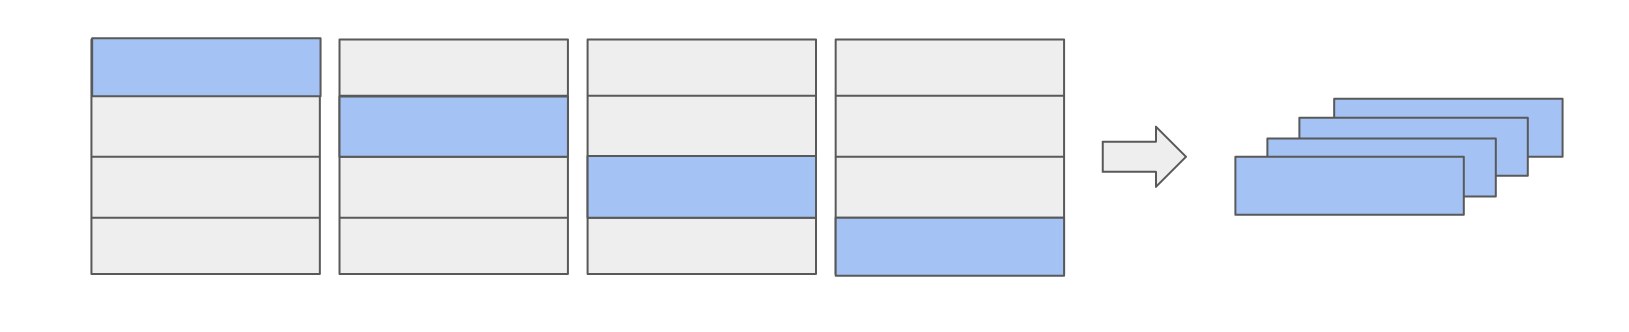
\includegraphics[scale=0.3]{img_3.png}
\end{figure}
        \subitem- \textbf{N Component:} the images of the full corpus are stacked.
        \begin{figure}[h!]
    \centering
    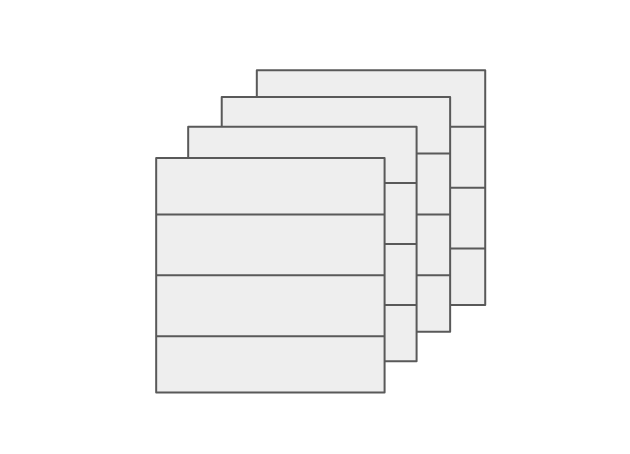
\includegraphics[scale=0.3]{img_2.png}
\end{figure}
    \item Modifications have been performed on each corpus separately and with all the images together. In all cases the results shown are the average of each modified dataset, except for N component experiment where all the corpus images are treated as one.
    \item The best datasets for each codifier are indicated in blue
    
\end{enumerate}
\newpage

\section*{Result tables Boats}
\subsection*{Compression Ratio}
\begin{table}[h]
\begin{tabular}{lcccc}
\rowcolor[HTML]{C0C0C0} 
 & Original & Bands & Moving bands & N component \\
\cellcolor[HTML]{C0C0C0}Entropy & \cellcolor[HTML]{E0E0E0} 6.1480 &  \cellcolor[HTML]{E0E0E0} 6.1480 &  \cellcolor[HTML]{E0E0E0} 6.2968 &  \cellcolor[HTML]{E0E0E0} 6.5575\\ 
\cellcolor[HTML]{C0C0C0}CCSDS\_LCNL & 2.6552 & 2.6552 & 2.5666 & \cellcolor[HTML]{DAE8FC}2.6932  \\
\cellcolor[HTML]{C0C0C0}JPEG\_LS    & \cellcolor[HTML]{DAE8FC}2.5979 & \cellcolor[HTML]{DAE8FC}2.5979 & 2.5227 & 2.5866  \\
\cellcolor[HTML]{C0C0C0}Kakadu      & \cellcolor[HTML]{DAE8FC}2.5750 & 2.5696 & 2.4898 & 2.5553  \\
\cellcolor[HTML]{C0C0C0}V2F W       & \cellcolor[HTML]{DAE8FC}2.1966 & \cellcolor[HTML]{DAE8FC}2.1966 & 2.0962 & 2.1663  \\
\cellcolor[HTML]{C0C0C0}V2F 2-West  & \cellcolor[HTML]{DAE8FC}2.1876 & \cellcolor[HTML]{DAE8FC}2.1876 & 2.0347 & 2.1293  \\
\cellcolor[HTML]{C0C0C0}V2F JLS     & \cellcolor[HTML]{DAE8FC}2.1843 & \cellcolor[HTML]{DAE8FC}2.1843 & 2.0792 & 2.1505  \\
\end{tabular}
\end{table}


\subsection*{bpppc}
\begin{table}[h]
\begin{tabular}{lcccc}
\rowcolor[HTML]{C0C0C0} 
 & Original & Bands & Moving bands & N component \\
\cellcolor[HTML]{C0C0C0}Entropy & \cellcolor[HTML]{E0E0E0} 6.1480 &  \cellcolor[HTML]{E0E0E0} 6.1480 &  \cellcolor[HTML]{E0E0E0} 6.2968 &  \cellcolor[HTML]{E0E0E0} 6.5575\\ 
\cellcolor[HTML]{C0C0C0}CCSDS\_LCNL & 3.0296 & 3.0296 & 3.1177 & \cellcolor[HTML]{DAE8FC}2.9704  \\
\cellcolor[HTML]{C0C0C0}JPEG\_LS    & \cellcolor[HTML]{DAE8FC}3.0926 & \cellcolor[HTML]{DAE8FC}3.0926 & 3.1716 & 3.0928  \\
\cellcolor[HTML]{C0C0C0}Kakadu      & \cellcolor[HTML]{DAE8FC}3.1228 & 3.1294 & 3.2137 & 3.1306 \\
\cellcolor[HTML]{C0C0C0}V2F W       & \cellcolor[HTML]{DAE8FC}3.6929 & \cellcolor[HTML]{DAE8FC}3.6929 & 3.8228 & \cellcolor[HTML]{DAE8FC}3.6929  \\
\cellcolor[HTML]{C0C0C0}V2F 2-West  & \cellcolor[HTML]{DAE8FC}3.7570 & \cellcolor[HTML]{DAE8FC}3.7570 & 3.9442 & \cellcolor[HTML]{DAE8FC}3.7570  \\
\cellcolor[HTML]{C0C0C0}V2F JLS     & \cellcolor[HTML]{DAE8FC}3.7200 & \cellcolor[HTML]{DAE8FC}3.7200 & 3.8554 & \cellcolor[HTML]{DAE8FC}3.7200  \\
\end{tabular}
\end{table}


\subsection*{Efficiency}
% Formula: \[-\sum_{i=0}^{255} p_ilog_2(p_i)\]
\begin{table}[h]
\begin{tabular}{lcccc}
\rowcolor[HTML]{C0C0C0} 
 & Original & Bands & Moving bands & N component \\
\cellcolor[HTML]{C0C0C0}Entropy & \cellcolor[HTML]{E0E0E0} 6.1480 &  \cellcolor[HTML]{E0E0E0} 6.1480 &  \cellcolor[HTML]{E0E0E0} 6.2968 &  \cellcolor[HTML]{E0E0E0} 6.5575\\ 
\cellcolor[HTML]{C0C0C0}CCSDS\_LCNL & \cellcolor[HTML]{DAE8FC}2.0330 & \cellcolor[HTML]{DAE8FC}2.0330 & 2.0200 & 2.2076  \\
\cellcolor[HTML]{C0C0C0}JPEG\_LS    & \cellcolor[HTML]{DAE8FC}1.9903 & \cellcolor[HTML]{DAE8FC}1.9903 & 1.9855 & 2.1202  \\
\cellcolor[HTML]{C0C0C0}Kakadu      & 1.9726 & 1.9685 & 1.9598 & \cellcolor[HTML]{DAE8FC}2.0946  \\
\cellcolor[HTML]{C0C0C0}V2F W       & 1.6788 & 1.6788 & 1.6486 & \cellcolor[HTML]{DAE8FC}1.7757  \\
\cellcolor[HTML]{C0C0C0}V2F 2-West  & 1.6677 & 1.6677 & 1.5996 & \cellcolor[HTML]{DAE8FC}1.7454  \\
\cellcolor[HTML]{C0C0C0}V2F JLS     & 1.6689 & 1.6689 & 1.6350 & \cellcolor[HTML]{DAE8FC}1.7627  \\
\end{tabular}
\end{table}


\newpage

\section*{Result tables Fields}
\subsection*{Compression Ratio}
\begin{table}[h]
\begin{tabular}{lcccc}
\rowcolor[HTML]{C0C0C0} 
 & Original & Bands & Moving bands & N component \\
\cellcolor[HTML]{C0C0C0}Entropy & \cellcolor[HTML]{E0E0E0} 6.3783&  \cellcolor[HTML]{E0E0E0} 6.3783&  \cellcolor[HTML]{E0E0E0} 6.2492&  \cellcolor[HTML]{E0E0E0} 6.5155\\ 
\cellcolor[HTML]{C0C0C0}CCSDS\_LCNL & 2.6327 & 2.6329 & 2.6027 & \cellcolor[HTML]{DAE8FC}2.7290  \\
\cellcolor[HTML]{C0C0C0}JPEG\_LS    & \cellcolor[HTML]{DAE8FC}2.5574 & \cellcolor[HTML]{DAE8FC}2.5574 & 2.5298 & 2.5561  \\
\cellcolor[HTML]{C0C0C0}Kakadu      & \cellcolor[HTML]{DAE8FC}2.5467 & 2.5408 & 2.5119 & 2.5379  \\
\cellcolor[HTML]{C0C0C0}V2F W       & \cellcolor[HTML]{DAE8FC}2.2563 & \cellcolor[HTML]{DAE8FC}2.2563 & 2.2305 & 2.2498  \\
\cellcolor[HTML]{C0C0C0}V2F 2-West  & \cellcolor[HTML]{DAE8FC}2.3360 & \cellcolor[HTML]{DAE8FC}2.3360 & 2.3036 & 2.3220  \\
\cellcolor[HTML]{C0C0C0}V2F JLS     & \cellcolor[HTML]{DAE8FC}2.2549 & \cellcolor[HTML]{DAE8FC}2.2549 & 2.2286 & 2.2475  \\
\end{tabular}
\end{table}


\subsection*{bpppc}
\begin{table}[h]
\begin{tabular}{lcccc}
\rowcolor[HTML]{C0C0C0} 
 & Original & Bands & Moving bands & N component \\
\cellcolor[HTML]{C0C0C0}Entropy & \cellcolor[HTML]{E0E0E0} 6.3783&  \cellcolor[HTML]{E0E0E0} 6.3783&  \cellcolor[HTML]{E0E0E0} 6.2492&  \cellcolor[HTML]{E0E0E0} 6.5155\\
\cellcolor[HTML]{C0C0C0}CCSDS\_LCNL & 3.0406 & 3.0404 & 3.0746 & \cellcolor[HTML]{DAE8FC}2.9314  \\
\cellcolor[HTML]{C0C0C0}JPEG\_LS    & \cellcolor[HTML]{DAE8FC}3.1296 & \cellcolor[HTML]{DAE8FC}3.1296 & 3.1628 & \cellcolor[HTML]{DAE8FC}3.1296  \\
\cellcolor[HTML]{C0C0C0}Kakadu      & \cellcolor[HTML]{DAE8FC}3.1429 & 3.1501 & 3.1855 & 3.1521  \\
\cellcolor[HTML]{C0C0C0}V2F W       & \cellcolor[HTML]{DAE8FC}3.5557 & \cellcolor[HTML]{DAE8FC}3.5557 & 3.5921 & \cellcolor[HTML]{DAE8FC}3.5557  \\
\cellcolor[HTML]{C0C0C0}V2F 2-West  & \cellcolor[HTML]{DAE8FC}3.4452 & \cellcolor[HTML]{DAE8FC}3.4452 & 3.4845 & \cellcolor[HTML]{DAE8FC}3.4452  \\
\cellcolor[HTML]{C0C0C0}V2F JLS     & \cellcolor[HTML]{DAE8FC}3.5594 & \cellcolor[HTML]{DAE8FC}3.5594 & 3.5960 & \cellcolor[HTML]{DAE8FC}3.5594  \\
\end{tabular}
\end{table}


\subsection*{Efficiency}
% Formula: \[-\sum_{i=0}^{255} p_ilog_2(p_i)\]
\begin{table}[h]
\begin{tabular}{lcccc}
\rowcolor[HTML]{C0C0C0} 
 & Original & Bands & Moving bands & N component \\
\cellcolor[HTML]{C0C0C0}Entropy & \cellcolor[HTML]{E0E0E0} 6.3783&  \cellcolor[HTML]{E0E0E0} 6.3783&  \cellcolor[HTML]{E0E0E0} 6.2492&  \cellcolor[HTML]{E0E0E0} 6.5155\\ 
\cellcolor[HTML]{C0C0C0}CCSDS\_LCNL & 2.0984 & 2.0985 & 2.0329 & \cellcolor[HTML]{DAE8FC}2.2226  \\
\cellcolor[HTML]{C0C0C0}JPEG\_LS    & 2.0384 & 2.0384 & 1.9760 & \cellcolor[HTML]{DAE8FC}2.0818  \\
\cellcolor[HTML]{C0C0C0}Kakadu      & 2.0299 & 2.0252 & 1.9620 & \cellcolor[HTML]{DAE8FC}2.0669  \\
\cellcolor[HTML]{C0C0C0}V2F W       & 1.7980 & 1.7980 & 1.7421 & \cellcolor[HTML]{DAE8FC}1.8323  \\
\cellcolor[HTML]{C0C0C0}V2F 2-West  & 1.8613 & 1.8613 & 1.7993 & \cellcolor[HTML]{DAE8FC}1.8911  \\
\cellcolor[HTML]{C0C0C0}V2F JLS     & 1.7968 & 1.7968 & 1.7406 & \cellcolor[HTML]{DAE8FC}1.8304  \\
\end{tabular}
\end{table}


\newpage
\section*{Result tables Full Dataset}
\subsection*{Compression Ratio}
\begin{table}[h]
\begin{tabular}{lcccc}
\rowcolor[HTML]{C0C0C0} 
 & Original & Bands & Moving bands & N component \\
\cellcolor[HTML]{C0C0C0}Entropy & \cellcolor[HTML]{E0E0E0}6.3622 &  \cellcolor[HTML]{E0E0E0}6.3622 &  \cellcolor[HTML]{E0E0E0}6.2515 &  \cellcolor[HTML]{E0E0E0} 6.5666\\ 
\cellcolor[HTML]{C0C0C0}CCSDS\_LCNL & 2.6343 & 2.6345 & 2.6041 & \cellcolor[HTML]{DAE8FC} 2.7273\\
\cellcolor[HTML]{C0C0C0}JPEG\_LS    & \cellcolor[HTML]{DAE8FC}2.5602 & \cellcolor[HTML]{DAE8FC}2.5602 & 2.5322 & 2.5582\\
\cellcolor[HTML]{C0C0C0}Kakadu      & \cellcolor[HTML]{DAE8FC}2.5486 & 2.5428 & 2.5135 & 2.5390\\
\cellcolor[HTML]{C0C0C0}V2F W       & \cellcolor[HTML]{DAE8FC}2.2522 & \cellcolor[HTML]{DAE8FC}2.2522 & 2.2276 & 2.2438\\
\cellcolor[HTML]{C0C0C0}V2F 2-West  & \cellcolor[HTML]{DAE8FC}2.3256 & \cellcolor[HTML]{DAE8FC}2.3256 & 2.2953 & 2.3074\\
\cellcolor[HTML]{C0C0C0}V2F JLS     & \cellcolor[HTML]{DAE8FC}2.2499 & \cellcolor[HTML]{DAE8FC}2.2499 & 2.2250 & 2.2404\\
\end{tabular}
\end{table}


\subsection*{bpppc}
\begin{table}[h]
\begin{tabular}{lcccc}
\rowcolor[HTML]{C0C0C0} 
 & Original & Bands & Moving bands & N component \\
\cellcolor[HTML]{C0C0C0}Entropy & \cellcolor[HTML]{E0E0E0}6.3622 &  \cellcolor[HTML]{E0E0E0}6.3622 &  \cellcolor[HTML]{E0E0E0}6.2515 &  \cellcolor[HTML]{E0E0E0} 6.5666\\ 
\cellcolor[HTML]{C0C0C0}CCSDS\_LCNL & 3.0398 & 3.0396 & 3.0732 & \cellcolor[HTML]{DAE8FC} 2.9332\\
\cellcolor[HTML]{C0C0C0}JPEG\_LS    & \cellcolor[HTML]{DAE8FC}3.1270 & \cellcolor[HTML]{DAE8FC}3.1270 & 3.1601 & \cellcolor[HTML]{DAE8FC}3.1270 \\
\cellcolor[HTML]{C0C0C0}Kakadu      & \cellcolor[HTML]{DAE8FC}3.1415 & 3.1487 & 3.1837 & 3.1507\\
\cellcolor[HTML]{C0C0C0}V2F W       & \cellcolor[HTML]{DAE8FC}3.5653 & \cellcolor[HTML]{DAE8FC}3.5653 & 3.5979 & \cellcolor[HTML]{DAE8FC}3.5653\\
\cellcolor[HTML]{C0C0C0}V2F 2-West  & \cellcolor[HTML]{DAE8FC}3.4670 & \cellcolor[HTML]{DAE8FC}3.4670 & 3.4994 & \cellcolor[HTML]{DAE8FC}3.4670\\
\cellcolor[HTML]{C0C0C0}V2F JLS     & \cellcolor[HTML]{DAE8FC}3.5706 & \cellcolor[HTML]{DAE8FC}3.5706 & 3.6030 & \cellcolor[HTML]{DAE8FC}3.5706\\
\end{tabular}
\end{table}


\subsection*{Efficiency}
% Formula: \[-\sum_{i=0}^{255} p_ilog_2(p_i)\]
\begin{table}[h]
\begin{tabular}{lcccc}
\rowcolor[HTML]{C0C0C0} 
 & Original & Bands & Moving bands & N component \\
\cellcolor[HTML]{C0C0C0}Entropy & \cellcolor[HTML]{E0E0E0}6.3622 &  \cellcolor[HTML]{E0E0E0}6.3622 &  \cellcolor[HTML]{E0E0E0}6.2515 &  \cellcolor[HTML]{E0E0E0} 6.5666\\ 
\cellcolor[HTML]{C0C0C0}CCSDS\_LCNL & 2.0938 & 2.0939 & 2.0293 & \cellcolor[HTML]{DAE8FC} 2.2386\\
\cellcolor[HTML]{C0C0C0}JPEG\_LS    & 2.0350 & 2.0350 & 1.9733 & \cellcolor[HTML]{DAE8FC} 2.0989\\
\cellcolor[HTML]{C0C0C0}Kakadu      & 2.0259 & 2.0212 & 1.9588 & \cellcolor[HTML]{DAE8FC} 2.0841\\
\cellcolor[HTML]{C0C0C0}V2F W       & 1.7897 & 1.7897 & 1.7357 & \cellcolor[HTML]{DAE8FC} 1.8418\\
\cellcolor[HTML]{C0C0C0}V2F 2-West  & 1.8477 & 1.8477 & 1.7883 & \cellcolor[HTML]{DAE8FC} 1.8940\\
\cellcolor[HTML]{C0C0C0}V2F JLS     & 1.7879 & 1.7879 & 1.7337 & \cellcolor[HTML]{DAE8FC} 1.8390\\
\end{tabular}
\end{table}


\end{document}
